\documentclass{article}

\PassOptionsToPackage{numbers,compress}{natbib}
\usepackage[main]{neurips_2026}

\usepackage[utf8]{inputenc}
\usepackage[T1]{fontenc}
\usepackage{hyperref}
\usepackage{url}
\usepackage{booktabs}
\usepackage{amsmath,amsfonts,amssymb}
\usepackage{nicefrac}
\usepackage{microtype}
\usepackage{xcolor}
\usepackage{graphicx}
\usepackage{tabularx}
\usepackage{multirow}
\usepackage{tikz}
\usetikzlibrary{arrows.meta,calc,positioning}
\hypersetup{
  colorlinks=true,
  linkcolor=black,
  citecolor=teal!65!black,
  urlcolor=blue!60!black
}

\newcommand{\uvt}{$(u,v,t)$}
\newcommand{\method}{Jewels}
\newcommand{\ours}{\method{}}
\newcommand{\R}{\mathbb{R}}
\newcommand{\good}{\textcolor{teal!65!black}{\textbf{pass}}}
\newcommand{\partialgate}{\textcolor{orange!85!black}{\textbf{partial}}}

\title{Speaking Jewels into Spacetime: A Concept-and-Feasibility Study of\\Native Text-to-Video Gaussian Programs}

\author{Anonymous authors}

\begin{document}

\maketitle

\begin{abstract}
Text-to-video systems usually generate a raster latent and decode it into frames. We investigate a
different target language: a video is cast directly as an irregular field of persistent,
anisotropic Gaussian Jewels in displayed spacetime $(u,v,t)$. Each Jewel carries geometry,
opacity, color, and a local color derivative; time-tilted support represents motion. The intended
generator speaks a hierarchical executable program---semantic scene and ownership tokens,
trajectory phrases, physical Jewel tokens, and continuous centroids---that an additive renderer
turns into video. This paper makes a bounded feasibility claim, not an open-vocabulary generation
claim. In controlled experiments, free spacetime tilt improves reconstruction in 9/9 matched runs
by $0.772$ dB (95\% CI $[0.573,0.971]$); a support-correct amortized encoder improves from $21.876$
to $22.628$ dB as training data grows from 12 to 120 videos; and a prompt-and-seed-only exact
compiler generates nine 72k-Jewel programs with correct prompt similarity above shuffled and null
controls in 9/9 cases and OpenCLIP top-1 in 8/9. A 0.54M-parameter autoregressive speaker learns the
program syntax and recognizes all three held-out paraphrase classes, but fails the stricter rendered
retrieval gate. The remaining bottleneck is explicit: current trajectory macros are source-backed.
The next conclusive experiment is to learn reusable, source-independent trajectory prototypes at
larger data and compute scale.
\end{abstract}

\section{Introduction}
\label{sec:intro}

A video can be treated as a stack of pixels, or as a continuous volume whose axes are horizontal
position, vertical position, and time. We ask whether a text-conditioned model can generate the
second object directly. Our primitive is a spacetime Gaussian Jewel: a colored, soft-support basis
function living in the displayed-video volume \uvt. A slanted Jewel intersects consecutive time
slices at different image positions, so motion is part of its geometry rather than a correspondence
computed after frames are generated.

This target is neither a codec nor a claim of compactness. Video Gaussian representations have
already been studied for reconstruction, processing, and compression
\cite{sun2024splatter,smolak2024vegas,wang2025gsvc,lee2025gaussianvideo,shah2026garv}. Our question is
different: can text select and compose persistent Gaussian operations as the \emph{native output}
of a generative model? Such a model would speak into a continuous volume, keep explicit state across
temporal windows, and eventually permit local edits by modifying a bounded set of primitives.

The hypothesis is attractive but easy to overstate. Reconstructing an existing video proves that
the representation can hold video, not that language can generate it. A prompt-conditioned
scaffold followed by an encoder proves semantic preservation, not native prompt-to-Jewel
generation. Retrieval of a whole fitted source field is also not generation. We therefore use
input-ownership audits and shuffled/null controls to isolate a narrower feasibility statement.

Figure~\ref{fig:architecture} shows both the demonstrated path and its missing component. At
inference, the demonstrated prompt-only path receives exactly a prompt and integer seed, produces a
typed plan, composes distinct foreground and background trajectory donors, expands local physical
tokens at continuous centroids, and renders an irregular 72k-Jewel field. However, its macro
dictionary is built from 18 fitted training fields. It does not retrieve a complete video, but it
does reuse source-backed trajectory programs. Replacing those macros with reusable,
source-independent prototypes is the central next gate.

\begin{figure*}[t]
  \centering
  \resizebox{0.96\textwidth}{!}{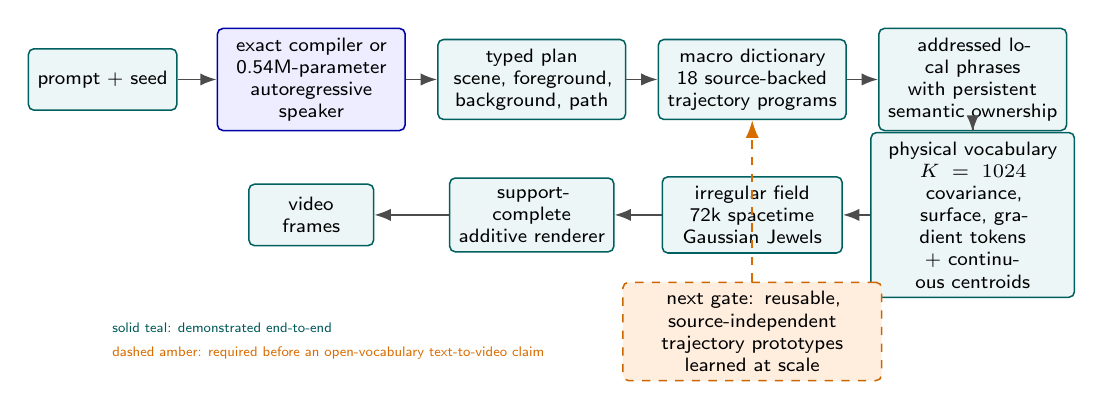
\begin{tikzpicture}[
  font=\sffamily\scriptsize,
  >=Latex,
  box/.style={draw=black!65, rounded corners=2pt, minimum height=0.78cm,
    text width=2.15cm, align=center, fill=white, line width=0.55pt},
  demonstrated/.style={box, fill=teal!7, draw=teal!75!black},
  speaker/.style={box, fill=blue!7, draw=blue!65!black},
  caution/.style={box, fill=orange!13, draw=orange!80!black, dashed},
  arrow/.style={->, line width=0.65pt, draw=black!70},
  next/.style={->, dashed, line width=0.75pt, draw=orange!85!black}
]
  \node[demonstrated, text width=1.65cm] (prompt) at (0,0) {prompt + seed};
  \node[speaker] (speaker) at (2.65,0) {exact compiler or\\0.54M-parameter\\autoregressive speaker};
  \node[demonstrated] (plan) at (5.45,0) {typed plan\\scene, foreground,\\background, path};
  \node[demonstrated] (macro) at (8.25,0) {macro dictionary\\18 source-backed\\trajectory programs};
  \node[demonstrated] (phrases) at (11.05,0) {addressed local phrases\\with persistent\\semantic ownership};
  \node[demonstrated, text width=2.35cm] (physical) at (11.05,-1.72) {physical vocabulary\\$K=1024$ covariance,\\surface, gradient tokens\\+ continuous centroids};
  \node[demonstrated, text width=2.05cm] (field) at (8.25,-1.72) {irregular field\\72k spacetime\\Gaussian Jewels};
  \node[demonstrated, text width=1.85cm] (render) at (5.45,-1.72) {support-complete\\additive renderer};
  \node[demonstrated, text width=1.35cm] (video) at (2.65,-1.72) {video\\frames};
  \node[caution, text width=3.05cm] (future) at (8.25,-3.2) {next gate: reusable, source-independent\\trajectory prototypes learned at scale};

  \draw[arrow] (prompt) -- (speaker);
  \draw[arrow] (speaker) -- (plan);
  \draw[arrow] (plan) -- (macro);
  \draw[arrow] (macro) -- (phrases);
  \draw[arrow] (phrases) -- (physical);
  \draw[arrow] (physical) -- (field);
  \draw[arrow] (field) -- (render);
  \draw[arrow] (render) -- (video);
  \draw[next] (future) -- (macro);

  \node[anchor=west, font=\sffamily\tiny, text=teal!70!black] at (0,-3.15)
    {solid teal: demonstrated end-to-end};
  \node[anchor=west, font=\sffamily\tiny, text=orange!85!black] at (0,-3.48)
    {dashed amber: required before an open-vocabulary text-to-video claim};
\end{tikzpicture}
}
  \caption{The proposed native text-to-video language. Solid boxes are demonstrated in this work;
  the dashed box is not. The exact compiler and learned speaker select a semantic plan, persistent
  foreground/background ownership, addressed phrases, and physical tokens. The crucial limitation
  is visible in the architecture: current macro tokens are backed by 18 fitted sources.}
  \label{fig:architecture}
\end{figure*}

Our contributions are:
\begin{itemize}
  \item a 22-parameter additive spacetime Gaussian primitive and a support-complete renderer that
  preserve continuous, irregular, time-tilted structure;
  \item causal and scaling evidence that temporal tilt is useful and that amortized video-to-Jewel
  prediction improves with data rather than collapsing to a coordinate grid;
  \item a hierarchical physical vocabulary with exact continuous centroids, three factorized
  $K=1024$ token books, and measurable same-source canonicality;
  \item a bounded prompt-and-seed-only test of this pipeline, including exact and learned
  speakers, complete input audits, negative controls, and an explicit failure of the learned
  speaker's strict rendered retrieval gate.
\end{itemize}

\section{Related work}

\paragraph{Dynamic and video Gaussians.}
3D Gaussian Splatting represents radiance fields with explicit anisotropic primitives
\cite{kerbl2023gaussians}. Dynamic extensions model time by deformation or native spacetime support
\cite{wu2024four,li2024spacetime}. Video-oriented methods use Gaussians for processing,
representation, or compression \cite{sun2024splatter,smolak2024vegas,wang2025gsvc,
lee2025gaussianvideo,shah2026garv}. These works establish that Gaussians can represent changing
visual signals. We focus on a displayed 2D video volume, additive rendering, and language-driven
construction rather than novel-view synthesis or rate-distortion performance.

\paragraph{Generative structured media.}
Video diffusion generates dense latent tensors \cite{ho2022video,blattmann2023stablevideo}.
Autoregressive multimodal models show that a language-modeling interface can emit visual tokens
\cite{chameleon2024,wang2024emu3}, while Transfusion combines discrete language modeling with
continuous visual generation \cite{zhou2025transfusion}. Gaussian generation has been explored for
3D and dynamic scenes \cite{zhang2024gaussiancube,roessle2024l3dg,lin2025diffsplat,pan2026diff4splat}.
Our proposal is complementary: the output tokens expand into persistent local operations in
displayed spacetime. The contribution is not next-token prediction for media, but an empirical
test of whether a hierarchical, executable Gaussian language has the required representational and
semantic properties.

\section{Method}

\subsection{A Jewel is a local function in displayed spacetime}

Let the normalized video domain be $\Omega=[-1,1]^3$, with query
$\mathbf{x}=(u,v,t)\in\Omega$. Jewel $i$ has center $\boldsymbol\mu_i\in\R^3$, symmetric positive
definite covariance $\boldsymbol\Sigma_i\in\R^{3\times3}$, opacity logit $\ell_i$, base RGB
$\mathbf{c}_i\in\R^3$, and local color Jacobian $\mathbf{J}_i\in\R^{3\times3}$. We evaluate
\begin{align}
q_i(\mathbf{x}) &= (\mathbf{x}-\boldsymbol\mu_i)^\top
  \boldsymbol\Sigma_i^{-1}(\mathbf{x}-\boldsymbol\mu_i), \\
a_i(\mathbf{x}) &= \sigma(\ell_i)\exp[-q_i(\mathbf{x})/2], \\
\widehat{\mathbf I}(\mathbf{x}) &= \mathbf b + \sum_i a_i(\mathbf{x})
  [\mathbf c_i+\mathbf J_i(\mathbf{x}-\boldsymbol\mu_i)],
\label{eq:render}
\end{align}
where $\mathbf b$ is a learned constant background. This is additive accumulation, not ordered
alpha compositing. The primitive has 22 continuous parameters: 3 center, 6 covariance, 1 opacity,
3 base-color, and 9 first-order color parameters. Values outside the display range are clipped only
for visualization; range violations are audited separately.

Writing $\boldsymbol\Sigma_i=\mathbf R_i\operatorname{diag}(\mathbf s_i^2)\mathbf R_i^\top$ makes
motion geometric. Off-diagonal space--time covariance tilts support into $t$; the intersection with
successive fixed-$t$ planes moves across $(u,v)$. Figure~\ref{fig:jewel} illustrates this without
the misleading picture of a flat frame translating laterally through image space.

\begin{figure}[t]
  \centering
  \resizebox{\linewidth}{!}{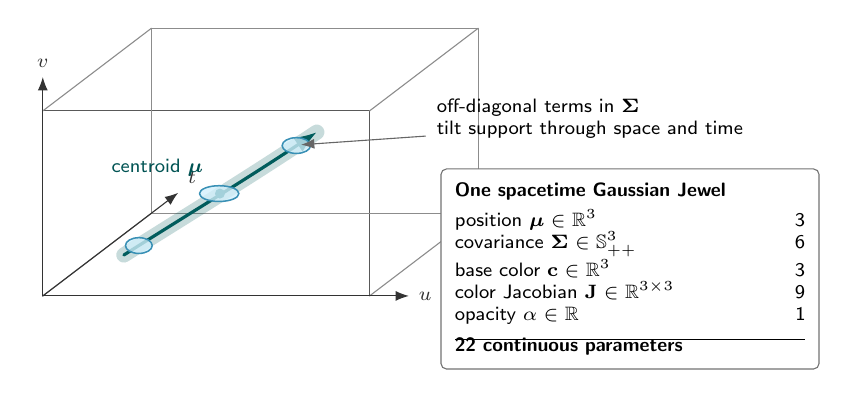
\begin{tikzpicture}[font=\sffamily\scriptsize, >=Latex, line cap=round, line join=round]
  % Spacetime volume.
  \coordinate (o) at (0,0);
  \coordinate (u) at (4.15,0);
  \coordinate (v) at (0,2.35);
  \coordinate (t) at (1.38,1.05);
  \draw[black!65] (o)--(u)--($(u)+(v)$)--(v)--cycle;
  \draw[black!45] (o)--(t) (u)--($(u)+(t)$) (v)--($(v)+(t)$) ($(u)+(v)$)--($(u)+(v)+(t)$);
  \draw[black!45] (t)--($(u)+(t)$)--($(u)+(v)+(t)$)--($(v)+(t)$)--cycle;
  \draw[->, black!80] (o) -- ++(4.65,0) node[right] {$u$};
  \draw[->, black!80] (o) -- ++(0,2.78) node[above] {$v$};
  \draw[->, black!80] (o) -- ++(1.72,1.31) node[above right] {$t$};

  % A tilted spacetime Jewel and three temporal cross-sections.
  \draw[teal!70!black, line width=5.5pt, opacity=.22] (1.03,.52) .. controls (1.82,1.02) and (2.58,1.48) .. (3.48,2.08);
  \draw[teal!72!black, line width=1.15pt, ->] (1.03,.52) .. controls (1.82,1.02) and (2.58,1.48) .. (3.48,2.08);
  \fill[teal!80!black] (2.25,1.30) circle (1.8pt);
  \node[anchor=south east, text=teal!65!black] at (2.16,1.39) {centroid $\boldsymbol\mu$};

  \foreach \x/\y/\r in {1.22/.64/.17,2.24/1.30/.25,3.22/1.91/.18}{
    \fill[cyan!18, opacity=.78] (\x,\y) ellipse (\r cm and .10cm);
    \draw[cyan!70!black, line width=.55pt] (\x,\y) ellipse (\r cm and .10cm);
  }
  \node[align=left, anchor=west] at (4.88,2.25) {off-diagonal terms in $\boldsymbol\Sigma$\\tilt support through space and time};
  \draw[->, black!60] (4.86,2.03) -- (3.28,1.92);

  % Parameter card.
  \node[draw=black!55, rounded corners=2pt, fill=white, align=left,
    text width=4.45cm, inner sep=5pt, anchor=north west] (card) at (5.05,1.62) {
      \textbf{One spacetime Gaussian Jewel}\par\smallskip
      position $\boldsymbol\mu\in\mathbb{R}^3$\hfill 3\\
      covariance $\boldsymbol\Sigma\in\mathbb{S}_{++}^3$\hfill 6\\
      base color $\mathbf c\in\mathbb{R}^3$\hfill 3\\
      color Jacobian $\mathbf J\in\mathbb{R}^{3\times3}$\hfill 9\\
      opacity $\alpha\in\mathbb{R}$\hfill 1\\[-1pt]
      \rule{\linewidth}{.35pt}\\[-4pt]
      \textbf{22 continuous parameters}
    };
\end{tikzpicture}
}
  \caption{One spacetime Gaussian Jewel. A video frame is a fixed-$t$ slice. The cross-section of
  tilted support changes position across slices, representing motion continuously. The color
  Jacobian permits local appearance change through space and time.}
  \label{fig:jewel}
\end{figure}

\subsection{Support-correct irregular rendering}

The original fast renderer selected a fixed number of Euclidean nearest centers. That shortcut can
silently omit wide or rotated Gaussians and confound a representation test with an approximation
artifact. Our support-complete renderer tiles query voxels, finds every primitive whose exact
Mahalanobis support lies within five standard deviations, and raises an error rather than dropping
contributors when capacity is exceeded. At 10k, 45k, and 72k primitives it runs within roughly
$2\times$ the k-nearest renderer; at 72k its measured peak allocation is 8.01 GB on an RTX 4090.
Pixels and gradients agree with dense evaluation up to the declared support truncation.

Irregularity is equally important. Centroids are continuous and jittered; local phrases do not
place one primitive on each fixed cell. We report the fraction of centers locked to the implied grid
and require zero. This separates a useful structured address from visible coordinate quantization.

\subsection{A hierarchical executable language}

A flat sequence of 72k independent 22-D records is too long and has no semantic ownership. We use
four levels:
\begin{enumerate}
  \item a \emph{scene token} chooses the semantic family;
  \item foreground and background \emph{owner tokens} keep coherent donors along a full
  space--time trajectory instead of switching independently per cell;
  \item addressed local phrases specify occupancy and which owner supplies each region; and
  \item three physical token books independently quantize covariance, surface/base color, and
  color gradient, while centers remain continuous.
\end{enumerate}
The factorization has $3\times1024$ active physical entries rather than a single combinatorial
codebook. An eight-frame field requires 35,265 discrete decisions, below a preregistered 40k-token
budget, and expands deterministically into an irregular field. The active representation reaches
22.866 dB token-only reconstruction PSNR, retains $1.042\times$ the teacher's median mixed
space--time tilt, and has zero grid locking. Same-source physical token overlap is 0.452 versus
0.228 for different sources, a 0.224 canonicality margin.

Persistent ownership emerged as the load-bearing abstraction. A global scene decoder and a purely
addressed $16\times16\times8$ local phrase model each produced zero recognizable classes, although
the local model improved token NLL from 6.123 to 5.168. Holding one coherent source through the
volume recovered 3/3 classes. Assigning one foreground donor and a different background donor along
a smoothed saliency trajectory preserved 3/3 and created a composition absent from any single
source. Thus locality improves syntax, but trajectory-level ownership carries semantics.

\subsection{Exact and learned speakers}

The \emph{exact compiler} maps three exact prompts and a seed to
$(\text{scene},\text{foreground owner},\text{background owner},\text{path})$. For each prompt, it
chooses two distinct donors from six fitted fields in that class, with exactly 50/50 primitive
ownership. The source choice is made once per temporal window, not independently per voxel. No
target video, target field, block program, or held-out latent is provided at inference.

The \emph{learned speaker} tests whether the plan has learnable syntax rather than only hand-written
dispatch. A 541,223-parameter autoregressive network conditions on a 512-D text embedding and emits
scene, foreground, then background tokens. It trains on 216 programs spanning each exact prompt and
two paraphrases per class; an unseen fourth phrasing is reserved for evaluation. This is a small
speaker over a closed three-scene vocabulary, not an LLM and not an open-vocabulary model.

\section{Experimental design}
\label{sec:experiments}

We organize experiments as falsifiable gates rather than a cumulative demo. Every positive semantic
claim includes a cyclic-shuffled prompt and a null-text control. Conditions share seeds and, where
applicable, weights and targets. Prompt similarity is measured with OpenCLIP ViT-B/32
\cite{radford2021clip}; reconstruction uses PSNR and LPIPS \cite{zhang2018lpips}. CLIP is used as a
screening metric, not as evidence of human-perceived video quality.

\paragraph{Causal representation test.}
We fit free full-covariance Jewels and a matched control whose space--time covariance is projected to
zero after every update. Primitive count, parameter bytes, initialization family, and optimization
budget are matched across three source videos and three seeds. We report paired differences and a
two-sided Student-$t$ 95\% interval over the nine pairs.

\paragraph{Data scaling test.}
An amortized 5.26M-parameter encoder is trained on exact nested subsets of 12, 60, or 120 examples
from five styles and 12 actions. Each budget has three independent seeds and is evaluated on the
same frozen 60-video inventory. Models receive 120 matched corpus passes and a common low-rate
continuation. Confidence intervals are $t$ intervals over the three seed means; no arm is selected
at a different exposure count. The fitted per-video teacher is an empirical ceiling, not a
comparable generalizing model.

\paragraph{Prompt-only test.}
The exact compiler is evaluated on ballerina, dog, and welder prompts, three seeds each. Each output
contains 72k Jewels and renders 49 frames at $144\times216$. Success requires that correct-prompt
similarity exceed both shuffled and null controls for every program, with at least 6/9 strict
OpenCLIP top-1 outcomes and majority success for all classes. The learned speaker uses the same
render audit on unseen paraphrases; its weights are frozen at the best held-out correct-text NLL
checkpoint before generating videos.

\section{Results}

\begin{table*}[t]
\centering
\caption{Evidence ledger. Pass means the declared bounded gate passed; it does not extend the
scope stated in the final column. Exact per-run values are retained in machine-readable reports.}
\label{tab:evidence}
\small
\begin{tabularx}{\textwidth}{@{}p{2.55cm}p{3.05cm}Xcp{3.35cm}@{}}
\toprule
Question & Control & Result & Gate & What it establishes \\
\midrule
Does time tilt help? & Full covariance vs. zeroed space--time terms; matched resources &
Free wins 9/9; $+0.772$ dB, 95\% CI $[0.573,0.971]$ & \good &
Space--time covariance is causally useful on the tested reconstructions. \\
Does the encoder scale? & Nested 12/60/120 sets, 3 seeds, fixed 60-video validation &
$21.876\rightarrow22.399\rightarrow22.628$ dB; LPIPS $0.473\rightarrow0.465\rightarrow0.392$ & \good &
More data improves held-out prediction under matched protocol. \\
Is the physical language irregular and faithful? & Token-only decode; grid-lock and tilt audits &
22.866 dB; zero grid lock; $1.042\times$ tilt; 0.224 canonicality margin & \good &
Factorized tokens preserve physical structure with exact centroids. \\
Can prompt + seed select video? & 9 correct/shuffled/null programs; no target artifact at inference &
Correct beats both controls 9/9; strict top-1 8/9; all class majorities & \good &
A bounded source-backed native program is prompt-selective. \\
Can a small speaker generalize phrasing? & Unseen fourth paraphrase; frozen checkpoint; same render audit &
Scene accuracy 3/3; NLL 2.201 vs. 4.387 shuffled; rendered top-1 4/9 & \partialgate &
Program syntax is learnable; rendered open-ended generalization is not established. \\
\bottomrule
\end{tabularx}
\end{table*}

\subsection{Temporal tilt is useful, not decorative}

The free model beats the projected control in all nine paired fits. The mean paired PSNR gain is
0.77197 dB (sample standard deviation 0.25858 dB; 95\% CI $[0.57321,0.97072]$). Median mixed
space--time tilt is 0.3459 in the free models and exactly zero by construction in controls. Gains are
larger on higher-motion sources. Because primitive counts and serialized parameter bytes are
matched, the result is evidence for the orientation of support, not extra capacity. It does not
prove that every video benefits or that the current parameterization is optimal.

\subsection{The amortized bottleneck improves with data}

Figure~\ref{fig:scaling} reports the predeclared scaling study. Mean held-out PSNR improves at both
budget increases: 21.876 dB (95\% CI $[21.751,22.000]$), 22.399 dB
($[22.344,22.453]$), and 22.628 dB ($[22.459,22.797]$). Every 120-example seed beats every
60-example seed. From 60 to 120 examples, LPIPS falls 15.8\%, layout PSNR rises from 30.726 to
31.533 dB, and median mixed tilt grows $2.58\times$ from 0.0725 to 0.1875. The fitted teacher ceiling
is 27.699 dB, LPIPS 0.1720, and median tilt 0.3966, leaving substantial headroom.

\begin{figure}[t]
  \centering
  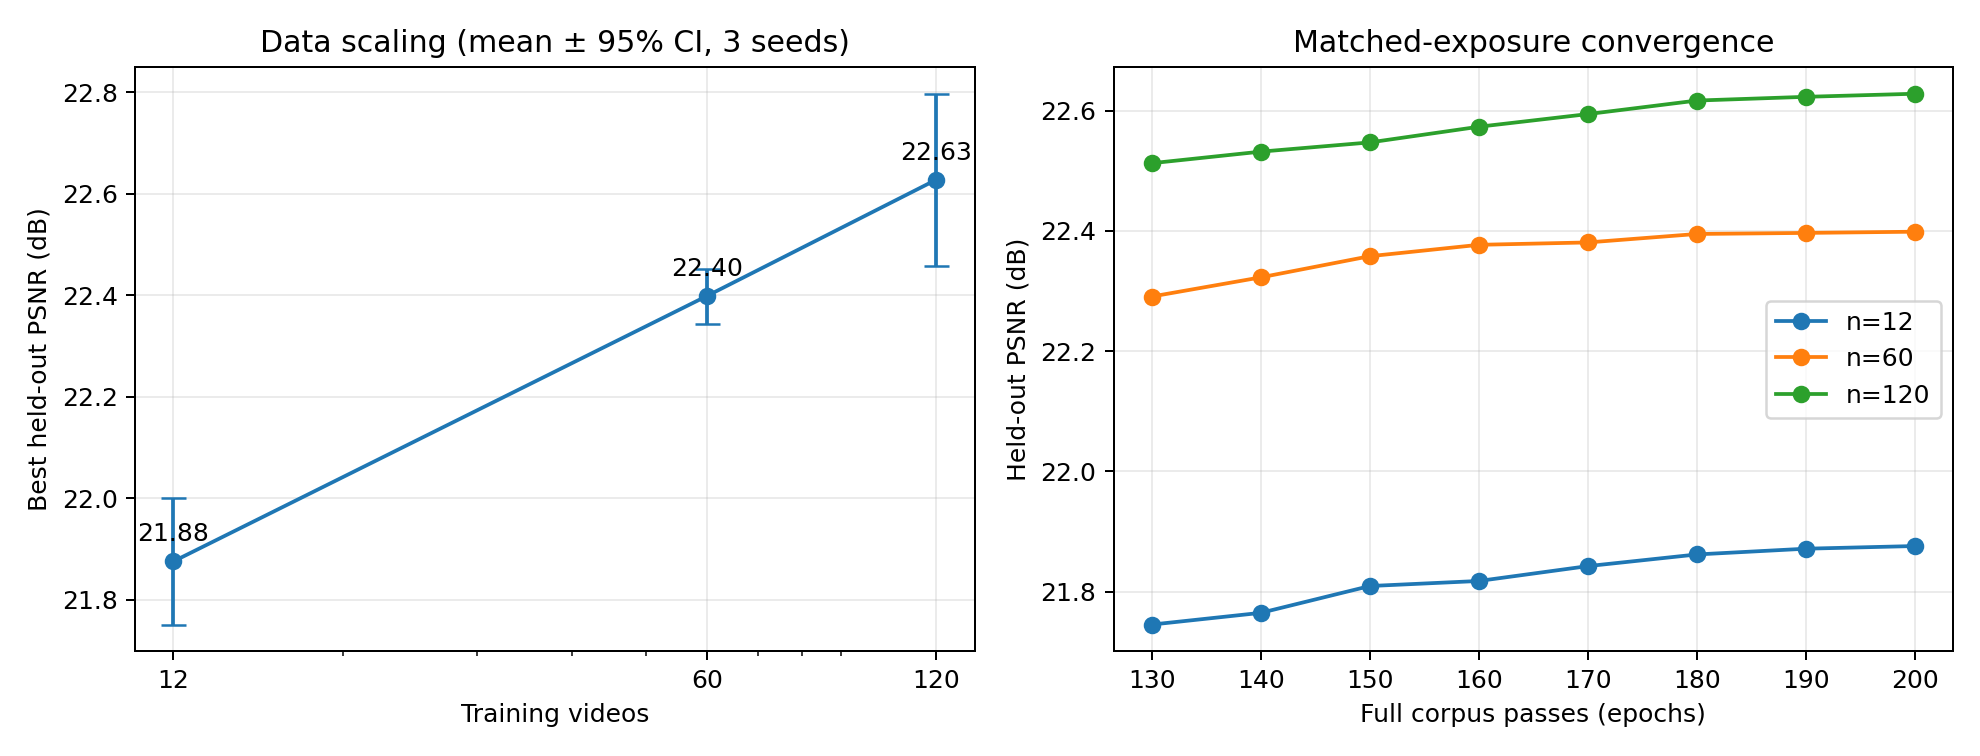
\includegraphics[width=\linewidth]{../../sol/results/encoder_convergence_v2_continued/aggregate/convergence.png}
  \caption{Support-correct encoder scaling. Left: held-out PSNR against training-set size, mean and
  95\% $t$ interval over three seeds. Right: convergence against matched corpus exposure. The trend
  supports a data-and-compute scaling hypothesis but remains a small-data study.}
  \label{fig:scaling}
\end{figure}

The same encoder preserves prompt information through a conservative
text-to-pretrained-video-to-encoder route: correct prompt similarity is 0.3339 versus 0.1427
shuffled and 0.2096 null on 12 held-out actions. Correct beats shuffled in 12/12 cases and retains
91.4\% of the source video's prompt alignment. This is useful evidence that the representation does
not erase semantics, but it is deliberately excluded from the native-generation claim because a
pretrained video model supplies the source video.

\subsection{The exact prompt-only compiler passes its bounded gate}

Across nine programs, mean OpenCLIP similarity is 0.18173 for the correct prompt, 0.12525 for the
cyclic-shuffled prompt, and 0.14825 for null text. The paired margins are $+0.05648$ and $+0.03348$;
correct exceeds each control for all 9/9 programs. Strict top-1 is 8/9 and majority retrieval passes
for all three classes. Foreground and background donor identifiers are distinct in every program,
ownership is exactly balanced, and grid-lock fraction is zero. The input audit confirms that the
only semantic inputs are exact prompt text and the declared integer seed.

Figure~\ref{fig:qualitative} shows all conditions rather than selected successes. The exact compiler
is visibly class-selective and composes donor regions, but quality is far below a modern dense video
generator. Because the macro vocabulary is source-backed, this result establishes execution and
semantic selection, not novel open-vocabulary motion.

\begin{figure}[t]
  \centering
  \begin{minipage}[t]{0.49\linewidth}
    \centering
    \textbf{Exact prompt compiler}\\[-2pt]
    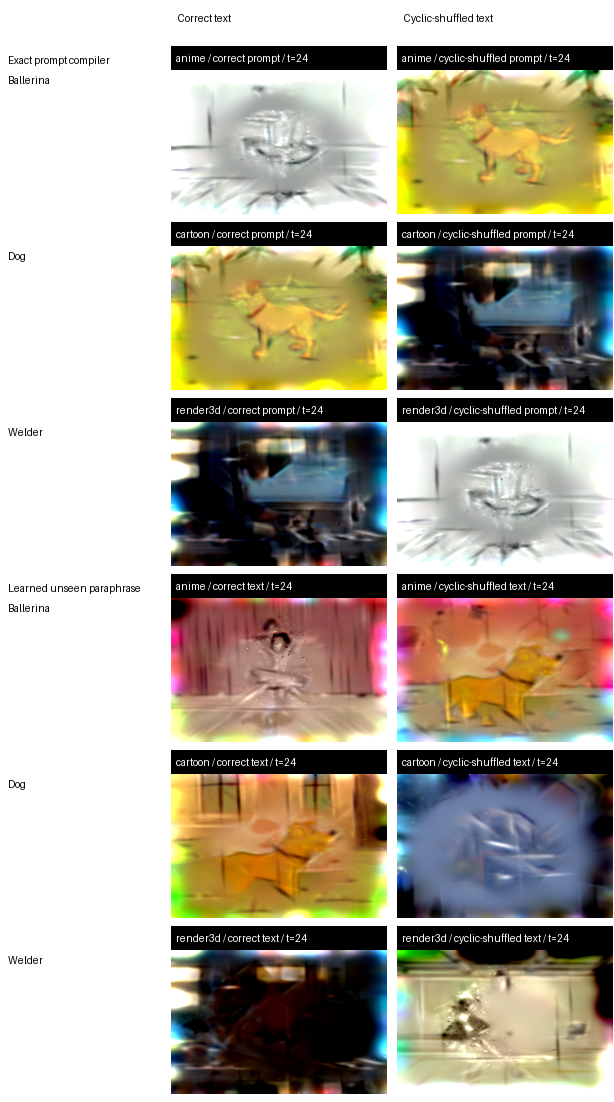
\includegraphics[width=\linewidth,trim={145bp 551bp 8bp 0bp},clip]{../../sol/results/jewel_casting_language_v0/trajectory_speaker_evidence_v1/trajectory_speaker_proof_sheet.png}
  \end{minipage}\hfill
  \begin{minipage}[t]{0.49\linewidth}
    \centering
    \textbf{Learned unseen paraphrase}\\[-2pt]
    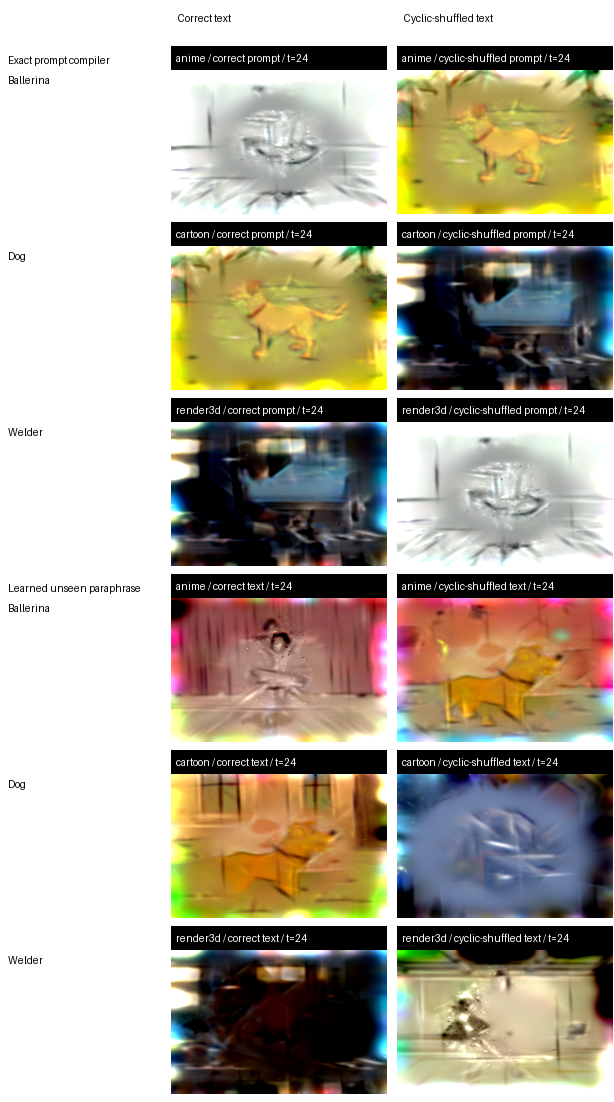
\includegraphics[width=\linewidth,trim={145bp 0bp 8bp 575bp},clip]{../../sol/results/jewel_casting_language_v0/trajectory_speaker_evidence_v1/trajectory_speaker_proof_sheet.png}
  \end{minipage}
  \caption{Prompt-only proof sheet reflowed from one audited image. Each half shows correct-prompt
  and cyclic-shuffled generation for ballerina, dog, and welder classes. All evaluated samples are
  shown. These are 72k-Jewel renders, not source frames; their trajectory macro tokens are
  nevertheless backed by fitted training fields.}
  \label{fig:qualitative}
\end{figure}

\subsection{The learned speaker exposes the next bottleneck}

The learned speaker reaches its best held-out correct-text NLL at step 100 and continues to step
1100 before the declared plateau rule stops training. On unseen paraphrases, macro token NLL is
2.2005 for correct text, 4.3870 for shuffled text, and 2.5391 for null text. Scene accuracy is 100\%
for correct text, 0\% shuffled, and 33\% null; all nine correct-text samples are scene-consistent.
In rendered space, correct similarity exceeds shuffled by 0.04782 on average and null by 0.04117,
with 7/9 correct-over-shuffled pairs.

The strict rendered top-1 test nevertheless passes only 4/9, below the declared 6/9 threshold, and
only one of three class majorities passes. This failure is informative but not an impossibility
result. The network learned the coarse scene syntax under unseen wording; it did not reliably
choose fine donor combinations whose low-fidelity renders win a frozen semantic retrieval test.
More steps alone are not the leading intervention because held-out correct NLL plateaued early. The
next experiment should change the vocabulary and supervision: learn reusable trajectory prototypes
from many sources, train the speaker against rendered semantic and temporal objectives, and compare
against a parameter-matched direct continuous head.

\section{What should scale next?}
\label{sec:scaling}

The experiments isolate three different scaling questions.

\paragraph{Representation compute.}
Longer local appearance optimization materially improves the frozen-geometry derivative head. For
one seed, LPIPS falls from 0.717 at 400 updates to 0.670 at 4k and 0.659 at 12k; a second seed reaches
0.660 at 12k. The final seeds differ by only 0.00058 LPIPS and 0.00041 dB PSNR, and geometry remains
bit-identical. This supports additional compute for appearance refinement, but diminishing returns
after roughly 8--12k updates argue against presenting optimization duration as the main missing
idea.

\paragraph{Encoder data.}
The monotone held-out curve and remaining teacher gap support a larger paired video/Jewel corpus.
The current 120-example maximum is far too small for a foundation model claim. A useful next scale
study should fix architecture and corpus passes, increase data by at least another order of
magnitude, and measure perceptual fidelity, layout, mixed tilt, and prompt retention jointly.

\paragraph{Generative vocabulary.}
This is the decisive axis. We propose segmenting many fitted fields into persistent trajectory tubes
using motion and semantic features, learning a dictionary whose entries aggregate across source
videos, and holding out entire motions, appearances, and compositions. A speaker should emit
prototype identities plus continuous transforms and residuals; a local flow or diffusion head can
model residual 22-D marks \cite{lipman2023flow,ludke2024pointset,hui2025notsoptimal}. The conclusive
pitch experiment is not merely prettier reconstruction. It is a prompt-only render whose every
macro token is source-independent, whose prompt and motion are held out compositionally, and whose
correct/shuffled/null margins persist over many classes and seeds.

\section{Limitations}
\label{sec:limitations}

\textbf{Closed semantic domain.} The prompt test contains three classes and 18 source fields. It
does not measure open vocabulary, long-form prompting, camera control, or physical interaction.

\textbf{Source-backed macro vocabulary.} Foreground and background trajectories reuse programs
derived from fitted sources. Although no whole video is retrieved and two donors are composed, the
system has not learned source-independent motion concepts. This is the principal limitation.

\textbf{Small, synthetic evaluation.} OpenCLIP retrieval is noisy at the current visual quality and
does not replace human judgment, FVD \cite{unterthiner2018fvd}, or a broad action benchmark. The
reported confidence intervals cover seeds within fixed small datasets, not dataset uncertainty.

\textbf{Rendering and color.} Additive overlap can wash out or overshoot RGB range, and the renderer
does not model occlusion through ordered alpha compositing. Support truncation is exact only with
respect to the declared five-sigma approximation.

\textbf{No demonstrated efficiency advantage.} We do not claim that a Jewel video is smaller,
cheaper, or higher quality than a latent video. A 72k-by-22 continuous field is not intrinsically a
compression format. The motivation is persistent executable structure; editing and scaling
advantages remain hypotheses requiring direct baselines.

\textbf{Negative experiments are local evidence.} Failure of a particular global decoder, local
phrase model, or learned retrieval gate identifies a missing dependency under its tested data and
optimizer. A single failed run is not treated as a law about Gaussian languages.

\section{Broader impact}
\label{sec:impact}

An explicit spacetime program could enable inspectable animation tools, localized corrections, and
reuse of persistent state. If future models make local edits without regenerating an entire video,
they may reduce iteration cost. The same capability can enable deceptive synthetic media,
impersonation, or biased visual depictions; explicit primitives do not remove those harms. Before
releasing a capable open-ended generator, appropriate measures include provenance metadata,
watermarking where robust, prompt and output abuse screening, consent-aware data curation, bias and
identity audits, and staged access. Training and rendering also consume energy. Efficiency claims
should be based on measured end-to-end quality-matched compute, not primitive counts alone.

\section{Conclusion}

The evidence supports a specific proposition: persistent time-tilted Gaussian Jewels form a useful
video basis, their amortized prediction improves with data, their physical parameters admit an
irregular hierarchical tokenization, and prompt plus seed can drive a bounded native program with
controlled semantic selectivity. It does not yet support the claim that we have a general
text-to-video model. The gap is sharply defined rather than mysterious: replace source-backed
trajectory macros with reusable learned prototypes, then demonstrate compositional prompt-only
generation on held-out motions and appearances. That experiment is the shortest path from a
convincing feasibility result to a compute-and-data scaling proposal.

\bibliographystyle{plainnat}
\bibliography{../references}

\appendix

\section{Protocols and preregistered gates}
\label{app:protocols}

\paragraph{Temporal-tilt gate.}
The inventory contains three source videos and seeds 0, 1, and 2. Free and projected models share
primitive and serialized parameter counts. The projection zeroes covariance entries $(u,t)$ and
$(v,t)$ after each optimizer step. The gate requires a positive mean paired PSNR difference, a 95\%
interval excluding zero, and removal of measured mixed tilt in the control.

\paragraph{Encoder-scaling gate.}
Nested train sets contain 12, 60, and 120 examples. The common validation set contains 60 examples
and has SHA-256 digest
\texttt{3e034a1263e21b566c79b63a8257e9794c4c66316e3a82d6fe65d418d1699b25}.
The encoder uses 4,096 sampled query points per step, AdamW, an initial matched 120-corpus-pass phase,
and a continuation at learning rate $3\times10^{-5}$ for at least 40 and at most 80 additional
passes. Evaluation occurs every 10 passes, with patience 3 and minimum improvement 0.03 dB. The
reported endpoint is the common continuation protocol, not per-arm cherry-picked training length.

\paragraph{Physical-language gate.}
The active books contain 1024 entries for covariance, 1024 for base/surface color, and 1024 for the
color Jacobian. Centers are not quantized. Required checks include finite metrics, token-only PSNR
above 20 dB, mixed-tilt retention above 0.8, exactly zero grid locking, fewer than 40k decisions for
eight frames, and same-source canonicality margin above 0.05.

\paragraph{Prompt-only gate.}
The exact prompts are a ballerina spinning a pirouette in a studio, a golden retriever catching a
ball on grass, and a welder joining steel with bright sparks. Seeds are 20260914, 20260915, and
20260916. Controls cyclically rotate prompts or remove text while holding the declared seed. The
learned speaker trains on each exact prompt and two paraphrases; a fourth paraphrase per class is
held out. Its AdamW learning rate is 0.002, batch size 64, text-dropout probability 0.1, minimum
1000 steps, maximum 5000 steps, evaluation interval 100, and plateau patience 10 evaluations with
minimum NLL improvement $10^{-4}$.

\section{Additional quantitative detail}

\begin{table}[ht]
\centering
\caption{Encoder scaling audit. Intervals are 95\% $t$ intervals over three seed means.}
\small
\begin{tabular}{@{}rrrrr@{}}
\toprule
Train videos & PSNR (dB) & 95\% CI & LPIPS & Layout PSNR \\
\midrule
12  & 21.876 & [21.751, 22.000] & 0.4728 & 29.812 \\
60  & 22.399 & [22.344, 22.453] & 0.4651 & 30.726 \\
120 & 22.628 & [22.459, 22.797] & 0.3916 & 31.533 \\
Teacher & 27.699 & -- & 0.1720 & -- \\
\bottomrule
\end{tabular}
\end{table}

\begin{table}[ht]
\centering
\caption{Prompt-only semantic audit. Similarities are OpenCLIP cosine values.}
\small
\begin{tabular}{@{}lrrr@{}}
\toprule
Speaker & Correct & Shuffled & Null \\
\midrule
Exact compiler & 0.18173 & 0.12525 & 0.14825 \\
Learned, unseen paraphrases & 0.25056 & 0.20274 & 0.20939 \\
\bottomrule
\end{tabular}
\end{table}

The learned speaker's higher absolute similarity is not evidence that it passes the stricter gate:
the relevant outcome is relative retrieval among candidate prompts for each generated sample. It
passes correct-over-shuffled in 7/9 cases but strict top-1 in only 4/9.

\section{Compute and implementation}
\label{app:compute}

Experiments ran on local NVIDIA RTX 4090 (24 GB) and RTX 2070 Super (8 GB) GPUs. Support-complete
72k-field rendering measured 8.01 GB peak allocation on the RTX 4090; chunked paths permit 45k--120k
field fitting on the 2070 Super. The encoder has 5.26M trainable parameters. Representative
12-example encoder continuations take approximately 129 seconds for 2,400 updates on the recorded
machine; larger arms scale with corpus size and evaluation cost. The learned speaker has 541,223
parameters and trains for 1,100 updates in the selected run. Derivative appearance studies run to
12k--16k updates. Total exploratory compute exceeds these selected runs because architectural
screening, renderer validation, and failed controls are retained in the repository rather than
omitted. A submission artifact should record exact GPU model, driver, package lock, wall time, and
energy estimate for every reproduced run.

\section{Reproducibility map}
\label{app:repro}

The following repository-relative machine-readable reports support the manuscript:
\begin{itemize}
  \item \path{sol/results/temporal_tilt_replication_v1/report.json};
  \item \path{sol/results/encoder_convergence_v2_continued/aggregate/report.json} and
    \path{audit/audit.json};
  \item \path{sol/results/jewel_casting_language_v0/hierarchical_v1/gate0f_individual/report.json};
  \item \path{sol/results/jewel_casting_language_v0/prompt_trajectory_speaker_v1/report.json};
  \item \path{sol/results/jewel_casting_language_v0/learned_trajectory_speaker_v1/report.json} and
    \path{audit/report.json}; and
  \item \path{sol/results/local_adapter_convergence_v1/README.md}.
\end{itemize}
Reports include protocol fields, artifact ownership, per-sample metrics, checks, and declared gate
outcomes. Code and reports are retained, but an anonymized public artifact with a complete license
audit has not yet been prepared; this is recorded as No in the checklist rather than implied.

\input{checklist}

\end{document}
